\documentclass[12pt]{article}
\usepackage{textcomp}
\usepackage{cmap}				    	% поиск в PDF
\usepackage{mathtext} 	           
\usepackage[T2A]{fontenc}			% кодировка
\usepackage[utf8]{inputenc}			% кодировка исходного текста
\usepackage[english]{babel}
\usepackage[colorlinks=true,urlcolor=darkgray,citecolor=darkgray,linkcolor=darkgray,bookmarks=true]{hyperref}
% \usepackage{ccaption}
\usepackage{authblk}
\usepackage{indentfirst}
% \usepackage{float} 
\usepackage{amsmath}
\usepackage{apacite}
\usepackage{natbib}
\usepackage{graphicx}
\usepackage{comment}
\usepackage{amsfonts}
\usepackage{bm}
\usepackage{amssymb}
\usepackage{amsthm}
\usepackage{mathtools}
\usepackage{upgreek} % AMS
\usepackage{marvosym}
\usepackage{threeparttable}
\usepackage{etoolbox}
\usepackage{cmap}	
\usepackage{multirow}
\usepackage{fullpage} 
\usepackage{geometry}
\geometry{
 a4paper,
 total={210mm,297mm},
 left=20mm,
 right=20mm,
 top=20mm,
 bottom=20mm,
 }
\usepackage{url}
\usepackage{pgfplots}
\usepackage{caption}
\usepackage{longtable}
\usepackage{multirow}
\usepackage{booktabs}
\usepackage{makecell}

\usepackage{pgf}
\usepackage{tikz}
\pgfplotsset{compat=1.15}
\usepackage{mathrsfs}
\usepackage{tikz} 
\usepackage{pgfplots}
\usepackage{pgfplotstable}
\usepackage{braket}
% \usepackage[capposition=top]{floatrow}
\usepackage{verbatim}
% \usepackage[position=bottom]{subfig}
\usepackage{graphicx}
%\usefonttheme[onlymath]{serif}
\usepackage[colorinlistoftodos]{todonotes}
\usepackage{setspace}% Интерлиньяж
\onehalfspacing % Интерлиньяж 1.5
%\doublespacing % Интерлиньяж 2
%\singlespacing % Интерлиньяж 1
\usepackage{econometrics}


\usepackage{appendix}



\usepackage{hyperref}
\usepackage{varioref}
\usepackage{cleveref}
\usepackage{fancyref}

\usepackage{csquotes} 



\usetikzlibrary{arrows}
\usetikzlibrary{calc}
\usetikzlibrary{positioning}
\usetikzlibrary{fit}
\usetikzlibrary{backgrounds}
\usetikzlibrary{intersections}
\tikzset{
style1/.style={
line cap=round,line join=round,
axis/.style={thick, ->, >=stealth'},
l/.style={thin},
d/.style={dashed, thin}, 
pile/.style={thin, <->, >=stealth',shorten <=3pt, shorten >=3pt}, 
every node/.style={color=black}, 
}
}





% \usepackage[backend=biber,
% style=chicago-authordate]{biblatex}
% \addbibresource{references.bib}

 \def\references{\bibliography{references.bib}
 \bibliographystyle{econ}}



\usepackage{parskip}

\setlength{\parindent}{15pt}
\setlength{\parskip}{5pt}

% \renewcommand{\maketitle}{\begin{center}
%         \noindent{\bfseries\scshape\Large\@title} 
%         \noindent{ \itshape\large\card{\subtitle}} 
%         \par  \vspace{0.5ex}
%         \noindent {\large\itshape\@author}
%         \noindent{\card{\footnotesize \itshape \extratext}}
%         \end{center}
%         } 

    % \makeatother
    % \def\extratext{}
    % \def\topic{}
    % \def\subtitle{}
       
 \newcommand{\card}[1]{ \ifthenelse{\equal{#1}{}}{}{ {\par#1}}}

 \usepackage{lipsum}

 \makeatletter
 \def\blfootnote{\gdef\@thefnmark{$\dagger$}\@footnotetext}
 \makeatother




    %%% Работа с картинками
    \usepackage{graphicx}  % Для вставки рисунков
    \setlength\fboxsep{3pt} % Отступ рамки \fbox{} от рисунка
    \setlength\fboxrule{1pt} % Толщина линий рамки \fbox{}
    \usepackage{wrapfig} % Обтекание рисунков текстом
    \usepackage{rotating}%поворот figure


    \DeclareRobustCommand{\firstsecond}[2]{#1}


    \makeatletter
\newcommand\footnoteref[1]{\protected@xdef\@thefnmark{\ref{#1}}\@footnotemark}
\makeatother


\usepackage{rotating}
% \usepackage{caption}
\usepackage{subcaption}
\captionsetup{labelfont=bf, labelsep=period, skip=0pt}


\pagestyle{plain}

\title{Local Governance and Natural Recourses}
\author{Alexander Vlasov\thanks{New Economic School. Email: avlasov@nes.ru.}}
\date{\normalsize First version: May, 2024\\\vspace{1ex} This version: May, 2024\\ \vspace{1ex}
\href{https:}{Click here for the most recent draft} }
\numberwithin{equation}{section}
\numberwithin{table}{section}
\numberwithin{figure}{section}


\begin{document}
\maketitle
\begin{abstract}
    123
\end{abstract}





\section{Empirical Methodology}



\begin{figure}\centering
    \caption{Municipalities by Governance Model}
    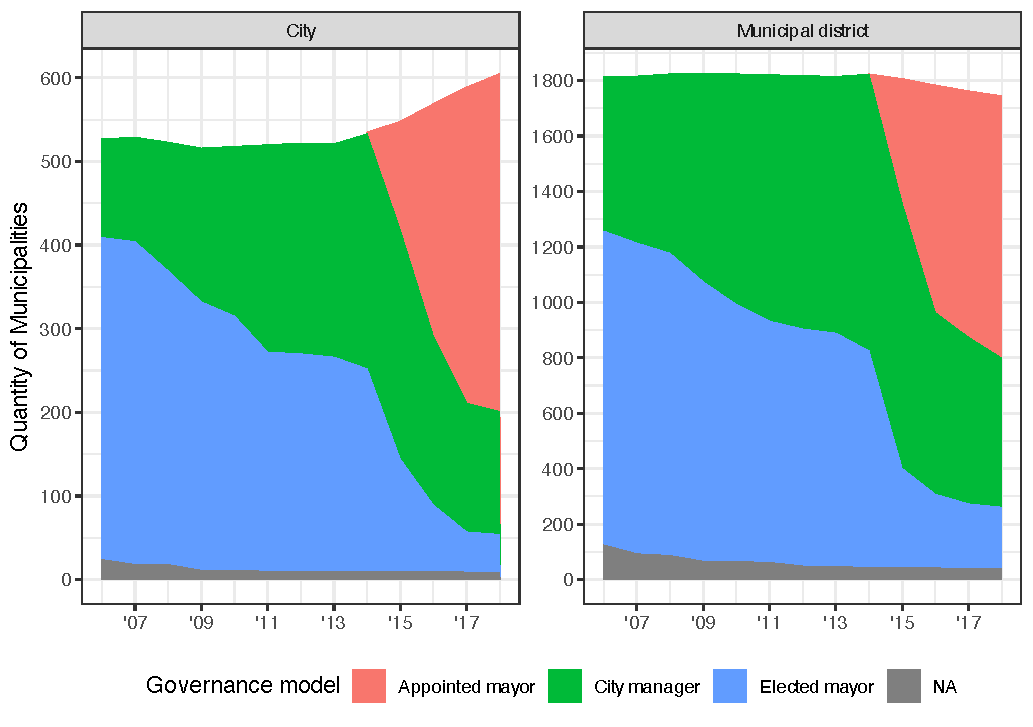
\includegraphics[width=\textwidth]{Figures/model_by_year_plot.pdf}
\end{figure}

\begin{figure}\centering
    \caption{Distributions of Regions by a Share of Municipalities with Elected Mayors by Year}
    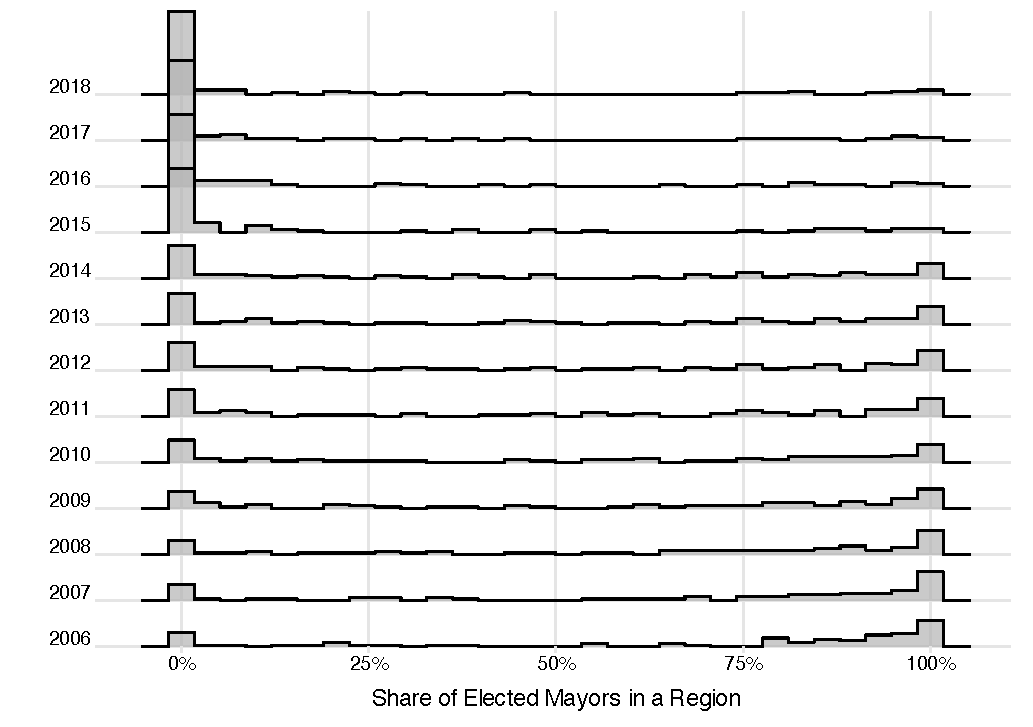
\includegraphics[width=\textwidth]{Figures/ridgeplot_models.pdf}
\end{figure}


\begin{figure}\centering
    \caption{Distribution of Regions by a Share of Municipalities with Elected Mayors}
    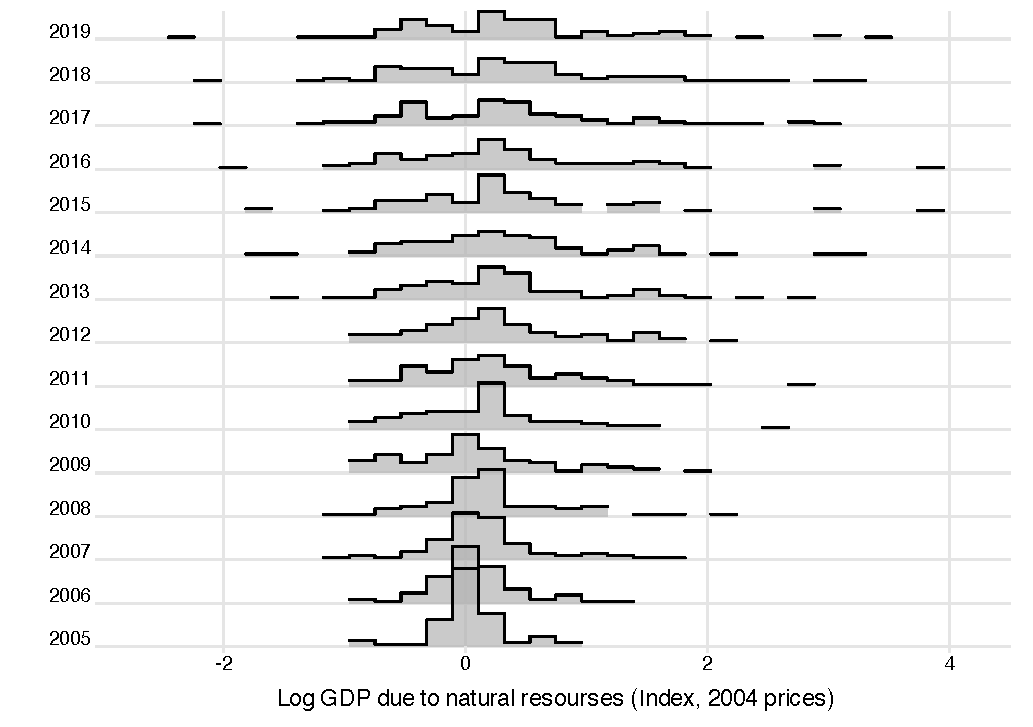
\includegraphics[width=\textwidth]{Figures/ridgeplot_resourse_extraction_gdp.pdf}
\end{figure}


\begin{table}[!htbp] \centering \footnotesize
\begin{threeparttable}
    \caption{} 
    \label{} 
  \begin{tabular}{@{\extracolsep{5pt}}lccc} 
  \\[-1.8ex]\hline 
  \hline \\[-1.8ex] 
   & \multicolumn{3}{c}{\textit{Dependent variable:}  (\%) Share of municipalities with} \\ 
  \cline{2-4} 
  \\[-1.8ex] & Elected Mayors & City Managers & Appointed Mayors\\ 
  \\[-1.8ex] $\log$ of& (1) & (2) & (3)\\ 
  \hline \\[-1.8ex]
  $\textit{Resourse Extraction GRDP}$ & 4.129$^{**}$ & $-$0.827 & $-$3.302 \\ 
  & (2.030) & (2.255) & (2.077) \\ 
  & & & \\ 
  $\textit{Energy GDRP}$ & 10.986$^{**}$ & 12.675$^{**}$ & $-$23.661$^{***}$ \\ 
  & (4.736) & (5.264) & (4.847) \\ 
  & & & \\ 
 $\textit{Military GDRP}$ & 16.178 & $-$26.434$^{**}$ & 10.256 \\ 
  & (10.917) & (12.132) & (11.172) \\ 
  & & & \\ 
 $\textit{Manufacturing GDRP}$ & $-$14.219$^{***}$ & 6.358 & 7.861$^{**}$ \\ 
  & (3.873) & (4.304) & (3.963) \\ 
  & & & \\ 
 $\textit{Healthcare GDRP}$ & 22.616 & $-$23.343 & 0.726 \\ 
  & (14.965) & (16.631) & (15.316) \\ 
  & & & \\ 
 $\textit{Education GDRP}$ & $-$31.483$^{**}$ & $-$16.380 & 47.863$^{***}$ \\ 
  & (13.381) & (14.871) & (13.695) \\ 
  & & & \\ 
 $\textit{Construction GDRP}$ & $-$4.229 & 10.379$^{***}$ & $-$6.150$^{**}$ \\ 
  & (2.778) & (3.087) & (2.843) \\ 
  & & & \\ 
 $\textit{Aggriculture GDRP}$ & $-$2.059$^{**}$ & 2.463$^{**}$ & $-$0.404 \\ 
  & (1.005) & (1.117) & (1.028) \\ 
  & & & \\ 
 $\textit{Retail GDRP}$ & 1.778 & $-$5.690 & 3.912 \\ 
  & (6.703) & (7.449) & (6.860) \\ 
  & & & \\ 
 $\textit{Transport GDRP}$ & $-$19.925$^{***}$ & 13.362$^{**}$ & 6.563 \\ 
  & (5.801) & (6.447) & (5.937) \\ 
  & & & \\ 
 $\textit{Hospitality GDRP}$& 13.735$^{***}$ & $-$3.600 & $-$10.135$^{**}$ \\ 
  & (4.168) & (4.632) & (4.266) \\ 
  & & & \\ 
  $\textit{GRDP}$ & 8.941 & $-$4.574 & $-$4.368 \\ 
  & (9.540) & (10.601) & (9.763) \\ 
  & & & \\ 
 $\textit{population}$ & 103.047$^{**}$ & $-$33.273 & $-$69.774$^{*}$ \\ 
  & (41.190) & (45.774) & (42.156) \\ 
  & & & \\ 
  Time-Region Fixed Effects & Yes& Yes& Yes \\
  \hline \\[-1.8ex] 
  $N$ & 976 & 976 & 976 \\ 
  $n$ & 77& 77& 77\\
  $T$ & 4--13 & 4--13& 4--13\\
  F Statistic & 5.703$^{***}$ & 3.449$^{***}$ & 4.690$^{***}$ \\ 
  \hline 
  \hline 
  \end{tabular} 
  \begin{tablenotes}[flushleft]
    \item \textit{Notes:} Double-clustering robust standard errors with HC3 influencial observations correction are in parenthesis \citep{Thompson2011,Cameron2011}. $^{*}\mathrm{p}<0.1$; $^{**}\mathrm{p}<0.05$; $^{***}\mathrm{p}<0.01$. Panel is unbalanced, $T=4$ for Crimea for which data is available from 2015 to 2018.
  \end{tablenotes}
\end{threeparttable}
  \end{table} 

\newpage 
\references


\appendix


\end{document}